% 유형 028 49-23(인쇄 49쪽) — 원 위에 같은 간격으로 놓인 8개의 점. 스캔 화질이 낮아 TikZ 로 다시 그림.
% 원문대로 점만 찍고 지름·삼각형은 그리지 않는다(직각삼각형의 개수가 그림에서 읽히지 않게). 라벨은 원문에 없다.
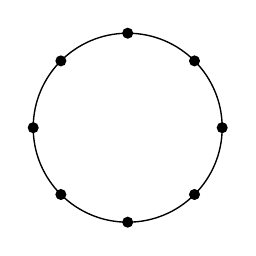
\begin{tikzpicture}[scale=1, line width=0.5pt]
  \draw (0,0) circle (1.2);
  \foreach \a in {0,45,...,315} { \fill (\a:1.2) circle (2pt); }
\end{tikzpicture}
